\chapter{Обзор} \label{chapt2}
Теория распознавания образа — раздел информатики и смежных дисциплин, развивающий основы и методы классификации и идентификации предметов, явлений, процессов, сигналов, ситуаций и т. п. объектов, которые характеризуются конечным набором некоторых свойств и признаков. Такие задачи решаются довольно часто, например, при переходе или проезде улицы по сигналам светофора. Распознавание цвета загоревшейся лампы светофора и знание правил дорожного движения позволяет принять правильное решение о том, можно или нельзя переходить улицу.

Необходимость в таком распознавании возникает в самых разных областях — от военного дела и систем безопасности до оцифровки аналоговых сигналов.

Проблема распознавания образа приобрела выдающееся значение в условиях информационных перегрузок, когда человек не справляется с линейно-последовательным пониманием поступающих к нему сообщений и в результате его голова переключается на режим одновременности восприятия и мышления, которому такое распознавание свойственно.

Неслучайно, таким образом, проблема распознавания образа оказалась в поле междисциплинарных исследований - в том числе в связи с работой по созданию искусственного интеллекта, а создание технических систем распознавания образа привлекает к себе всё большее внимание.

Распознавание образов — это отнесение исходных данных к определенному классу с помощью выделения существенных признаков, характеризующих эти данные, из общей массы несущественных данных.

Классическая постановка задачи распознавания образов: близка к постановке задачи классификации и предполагает наличие некоторого базового набора заранее известных классов (набор может расширятся), и образа (не обязательно визуального) которые надо классифицировать.

Наиболее часто в задачах распознавания визуальных образов рассматриваются монохромные изображения, что дает возможность рассматривать изображение как функцию на плоскости.

Множество же всех возможных функций f(x, y) на плоскости T — есть модель множества всех изображений X. Вводя понятие сходства между образами можно поставить задачу распознавания. Конкретный вид такой постановки сильно зависит от последующих этапов при распознавании в соответствии с тем или иным подходом.

В данной работе распознавание рассматривается в контексте задачи классификации. Можно выделить следующие классы алгоритмов для решения задачи классификации объектов.

\section{Распознавание текста}
Оптическое распознавание текста является исследуемой проблемой в областях распознавания образов, искусственного интеллекта и компьютерного зрения.

Системы оптического распознавания текста требуют калибровки для работы с конкретным шрифтом; в ранних версиях для программирования было необходимо изображение каждого символа, программа одновременно могла работать только с одним шрифтом. В настоящее время больше всего распространены так называемые «интеллектуальные» системы, с высокой степенью точности распознающие большинство шрифтов. Некоторые системы оптического распознавания текста способны восстанавливать исходное форматирование текста, включая изображения, колонки и другие нетекстовые компоненты.

Точное распознавание латинских символов в печатном тексте в настоящее время возможно только если доступны чёткие изображения, такие как сканированные печатные документы. Точность при такой постановке задачи превышает 99\%, абсолютная точность может быть достигнута только путем последующего редактирования человеком. Проблемы распознавания рукописного «печатного» и стандартного рукописного текста, а также печатных текстов других форматов (особенно с очень большим числом символов) в настоящее время являются предметом активных исследований.

Точность работы методов может быть измерена несколькими способами и поэтому может сильно варьироваться. К примеру, если встречается специализированное слово, не используемое для соответствующего программного обеспечения, при поиске несуществующих слов, ошибка может увеличиться.

Распознавание символов он-лайн иногда путают с оптическим распознаванием символов. Последний — это офф-лайн метод, работающий со статической формой представления текста, в то время как он-лайн распознавание символов учитывает движения во время письма. Например, в он-лайн распознавании, использующем PenPoint OS или планшетный ПК, можно определить, с какой стороны пишется строка: справа налево или слева направо.

Он-лайн системы для распознавания рукописного текста «на лету» в последнее время стали широко известны в качестве коммерческих продуктов. Алгоритмы таких устройств используют тот факт, что порядок, скорость и направление отдельных участков линий ввода известны. Кроме того, пользователь научится использовать только конкретные формы письма. Эти методы не могут быть использованы в программном обеспечении, которое использует сканированные бумажные документы, поэтому проблема распознавания рукописного «печатного» текста по-прежнему остается открытой. На изображениях с рукописным «печатным» текстом без артефактов может быть достигнута точность в 80\% — 90\%, но с такой точностью изображение будет преобразовано с десятками ошибок на странице. Такая технология может быть полезна лишь в очень ограниченном числе приложений.

Ещё одной широко исследуемой проблемой является распознавание рукописного текста. На данный момент достигнутая точность даже ниже, чем для рукописного «печатного» текста. Более высокие показатели могут быть достигнуты только с использованием контекстной и грамматической информации. Например, в процессе распознания искать целые слова в словаре легче, чем пытаться проанализировать отдельные символы из текста. Знание грамматики языка может также помочь определить, является ли слово глаголом или существительным. Формы отдельных рукописных символов иногда могут не содержать достаточно информации, чтобы точно (более 98\%) распознать весь рукописный текст.

Для решения более сложных проблем в сфере распознавания используются как правило интеллектуальные системы распознавания, такие как искусственные нейронные сети.

\section{Персептрон}
Ф. Розенблатт вводя понятие о модели мозга, задача которой состоит в том, чтобы показать, как в некоторой физической системе, структура и функциональные свойства которой известны, могут возникать психологические явления — описал простейшие эксперименты по различению. Данные эксперименты целиком относятся к методам распознавания образов, но отличаются тем, что алгоритм решения не детерминированный.

Простейший эксперимент, на основе которого можно получить психологически значимую информацию о некоторой системе, сводится к тому, что модели предъявляются два различных стимула и требуется, чтобы она реагировала на них различным образом. Целью такого эксперимента может быть исследование возможности их спонтанного различения системой при отсутствии вмешательства со стороны экспериментатора, или, наоборот, изучение принудительного различения, при котором экспериментатор стремится обучить систему проводить требуемую классификацию.

В опыте с обучением персептрону обычно предъявляется некоторая последовательность образов, в которую входят представители каждого из классов, подлежащих различению. В соответствии с некоторым правилом модификации памяти правильный выбор реакции подкрепляется. Затем персептрону предъявляется контрольный стимул и определяется вероятность получения правильной реакции для стимулов данного класса. В зависимости от того, совпадает или не совпадает выбранный контрольный стимул с одним из образов, которые использовались в обучающей последовательности, получают различные результаты:

Если контрольный стимул не совпадает ни с одним из обучающих стимулов, то эксперимент связан не только с чистым различением, но включает в себя и элементы обобщения.
Если контрольный стимул возбуждает некоторый набор сенсорных элементов, совершенно отличных от тех элементов, которые активизировались при воздействии ранее предъявленных стимулов того же класса, то эксперимент является исследованием чистого обобщения.

Персептроны не обладают способностью к чистому обобщению, но они вполне удовлетворительно функционируют в экспериментах по различению, особенно если контрольный стимул достаточно близко совпадает с одним из образов, относительно которых персептрон уже накопил определенный опыт.

Элементарный перцептрон состоит из элементов 3-х типов: S-элементов, A-элементов и одного R-элемента. S-элементы — это слой сенсоров, или рецепторов. В физическом воплощении они соответствуют, например, светочувствительным клеткам сетчатки глаза или фоторезисторам матрицы камеры. Каждый рецептор может находиться в одном из двух состояний — покоя или возбуждения, и только в последнем случае он передаёт единичный сигнал в следующий слой, ассоциативным элементам.

A-элементы называются ассоциативными, потому что каждому такому элементу, как правило, соответствует целый набор (ассоциация) S-элементов. A-элемент активизируется, как только количество сигналов от S-элементов на его входе превысило некоторую величину $\theta$. Таким образом, если набор соответствующих S-элементов располагается на сенсорном поле в форме буквы «Д», A-элемент активизируется, если достаточное количество рецепторов сообщило о появлении «белого пятна света» в их окрестности, то есть A-элемент будет как бы ассоциирован с наличием/отсутствием буквы «Д» в некоторой области.

Сигналы от возбудившихся $A$-элементов, в свою очередь, передаются в сумматор $R$, причём сигнал от i-го ассоциативного элемента передаётся с коэффициентом $w_{i}$. Этот коэффициент называется весом $A-R$ связи.

Так же как и $A$-элементы, $R$-элемент подсчитывает сумму значений входных сигналов, помноженных на веса (линейную форму). $R$-элемент, а вместе с ним и элементарный перцептрон, выдаёт <<1>>, если линейная форма превышает порог $\theta$, иначе на выходе будет <<-1>>. Математически, функцию, реализуемую $R$-элементом, можно записать так:

    $$f(x) = sign(\sum_{i=1}^{n} w_i x_i - \theta)$$

Обучение элементарного перцептрона состоит в изменении весовых коэффициентов $w_i$ связей $A-R$. Веса связей $S-A$ (которые могут принимать значения $\{-1; \theta; +1\}$) и значения порогов $A$-элементов выбираются случайным образом в самом начале и затем не изменяются. (Описание алгоритма см. ниже.)

После обучения перцептрон готов работать в режиме распознавания или обобщения. В этом режиме перцептрону предъявляются ранее неизвестные ему объекты, и перцептрон должен установить, к какому классу они принадлежат. Работа перцептрона состоит в следующем: при предъявлении объекта, возбудившиеся $A$-элементы передают сигнал $R$-элементу, равный сумме соответствующих коэффициентов $w_i$. Если эта сумма положительна, то принимается решение, что данный объект принадлежит к первому классу, а если она отрицательна — то ко второму.

\section{Алгоритмы обучения}
Важным свойством любой нейронной сети является способность к обучению. Процесс обучения является процедурой настройки весов и порогов с целью уменьшения разности между желаемыми (целевыми) и получаемыми векторами на выходе. В своей книге Розенблатт пытался классифицировать различные алгоритмы обучения перцептрона, называя их системами подкрепления.

Система подкрепления - это любой набор правил, на основании которых можно изменять с течением времени матрицу взаимодействия (или состояние памяти) перцептрона.

\subsection{Обучение с учителем}

Классический метод обучения перцептрона — это метод коррекции ошибки. Он представляет собой такой вид обучения с учителем, при котором вес связи не изменяется до тех пор, пока текущая реакция перцептрона остается правильной. При появлении неправильной реакции вес изменяется на единицу, а знак (+/-) определяется противоположным от знака ошибки.

Допустим, мы хотим обучить перцептрон разделять два класса объектов так, чтобы при предъявлении объектов первого класса выход перцептрона был положителен (+1), а при предъявлении объектов второго класса — отрицательным (−1). Для этого выполним следующий алгоритм:[5]

Случайным образом выбираем пороги для $A$-элементов и устанавливаем связи $S-A$ (далее они изменяться не будут).
Начальные коэффициенты $w_i$ полагаем равными нулю.
Предъявляем обучающую выборку: объекты (например, круги либо квадраты) с указанием класса, к которым они принадлежат.

Показываем перцептрону объект первого класса. При этом некоторые $A$-элементы возбудятся. Коэффициенты $w_i$, соответствующие этим возбуждённым элементам, увеличиваем на 1.

Предъявляем объект второго класса и коэффициенты $w_i$ тех $A$-элементов, которые возбудятся при этом показе, уменьшаем на 1.
    
Обе части шага 3 выполним для всей обучающей выборки. В результате обучения сформируются значения весов связей $w_i$.

Теорема сходимости перцептрона, описанная и доказанная Ф. Розенблаттом (с участием Блока, Джозефа, Кестена и других исследователей, работавших вместе с ним), показывает, что элементарный перцептрон, обучаемый по такому алгоритму, независимо от начального состояния весовых коэффициентов и последовательности появления стимулов всегда приведет к достижению решения за конечный промежуток времени.

\subsection{Обучение без учителя}

Кроме классического метода обучения перцептрона Розенблатт также ввёл понятие об обучении без учителя, предложив следующий способ обучения:

Альфа-система подкрепления - это система подкрепления, при которой веса всех активных связей $c_{ij}$, которые ведут к элементу $u_j$, изменяются на одинаковую величину $r$, а веса неактивных связей за это время не изменяются.

Затем, с разработкой понятия многослойного перцептрона, альфа-система была модифицирована и её стали называть дельта-правило. Модификация была проведена с целью сделать функцию обучения дифференцируемой (например, сигмоидной), что в свою очередь нужно для применения метода градиентного спуска, благодаря которому возможно обучение более одного слоя.

\subsection{Метод обратного распространения ошибки}

Для обучения многослойных сетей рядом учёных, в том числе Д. Румельхартом, был предложен градиентный алгоритм обучения с учителем, проводящий сигнал ошибки, вычисленный выходами перцептрона, к его входам, слой за слоем. Сейчас это самый популярный метод обучения многослойных перцептронов. Его преимущество в том, что он может обучить все слои нейронной сети, и его легко просчитать локально. Однако этот метод является очень долгим, к тому же, для его применения нужно, чтобы передаточная функция нейронов была дифференцируемой. При этом в перцептронах пришлось отказаться от бинарного сигнала, и пользоваться на входе непрерывными значениями.

\begin{figure}[h]
	\centering
	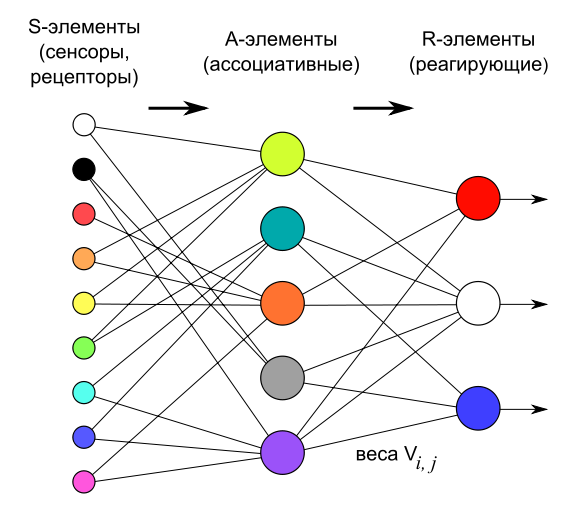
\includegraphics[height=4in]{images/intro_perceptron.png}
\end{figure}

\section{Поисковые системы}

\begin{enumerate}
\item 
\end{enumerate}
%Существует множество методов распознавания изображений но в целом их можно разделить на две группы:
%\begin{enumerate}
%\item эвристические
%\item формальные
%\end{enumerate}
%
%\section{Одиночное изображение} \label{sect2_1}
%
%\begin{figure} [h] 
%  \center
%  
\includegraphics [scale=0.27] {latex}
%  \caption{TeX.} 
%  \label{img:latex}  
%\end{figure}
%
%%\newpage
%%============================================================================================================================
%\section{Длинное название параграфа, в котором мы узнаём как сделать две картинки с общим номером и названием} \label{sect2_2}
%
%А это две картинки под общим номером и названием:
%\begin{figure}[h]
%  \begin{minipage}[h]{0.49\linewidth}
%    \center{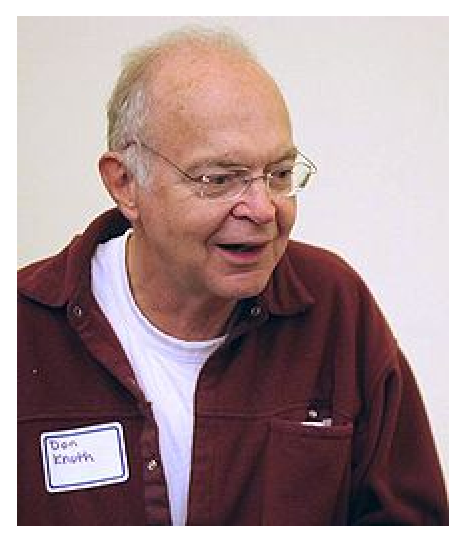
\includegraphics[width=0.5\linewidth]{knuth1} \\ а)}
%  \end{minipage}
%  \hfill
%  \begin{minipage}[h]{0.49\linewidth}
%    \center{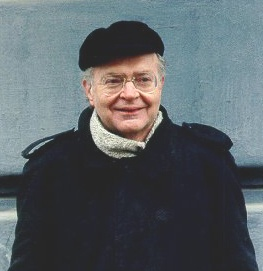
\includegraphics[width=0.5\linewidth]{knuth2} \\ б)}
%  \end{minipage}
%  \caption{Очень длинная подпись к изображению, на котором представлены две фотографии Дональда Кнута}
%  \label{img:knuth}  
%\end{figure}
%
%%\newpage
%%============================================================================================================================
%\section{Пример вёрстки списоков} \label{sect2_3}
%
%\noindent Нумерованный список:
%\begin{enumerate}
%  \item Первый пункт.
%  \item Второй пункт.
%  \item Третий пункт.
%\end{enumerate}
%
%\noindent Маркированный список:
%\begin{itemize}
%  \item Первый пункт.
%  \item Второй пункт.
%  \item Третий пункт.
%\end{itemize}
%
%\noindent Вложенные списки:
%\begin{itemize}
%  \item Имеется маркированный список.
%  \begin{enumerate}
%    \item В нём лежит нумерованный список,
%    \item в котором
%    \begin{itemize}
%      \item лежит ещё один маркированный список.
%    \end{itemize}    
%  \end{enumerate}
%\end{itemize}
%
%
%\clearpage